\documentclass[dvipdfmx]{beamer}

\usepackage{beamerthemesplit}
\usepackage[]{graphicx}
\graphicspath{%
{./slide07-img/}%
{./text07-img/}%
}

\usepackage{listings}
\usepackage{hyperref}
\usepackage{pxjahyper}
\usepackage{nameref} % これが\zexternaldocumentの前までに必要
\usepackage{zref-xr}
\usepackage{color}

\zxrsetup{toltxlabel} % 通常のLaTeXスタイルの\refを使う(\zexternaldocumentより前におく)
\zexternaldocument*[1:]{text07} % \zのついたexternaldocumentを使う

\setbeamertemplate{footline}[frame number]
\title{子どもIT未来塾 第7回}
\author{塾長 清水尚彦}

\def\quiz{1}

\begin{document}

\frame{
   \begin{center}
    \huge{子どもIT未来塾}\\

    \vspace{48pt}
	   \Large{第7回}\\
	   {\huge\bf ネットワークについて学ぼう}\\
    \vspace{24pt}
    \large{塾長 清水尚彦}\\
    \vspace{10pt}
    \large{\the\year 年 9月23日}
  \end{center}
}



\begin{frame}[fragile]
	\frametitle{3時間目 CGIをつかってみよう ~~~\raisebox{-3mm}{
\includegraphics[width=0.1\textwidth]{raspberry}}}
        \begin{itemize}
            \item CGI(Common Gateway Interface)プログラムを使うと、多機能なWebページを作ることができます。
        \end{itemize}
        \begin{minipage}{\textwidth}
            {\upshape
              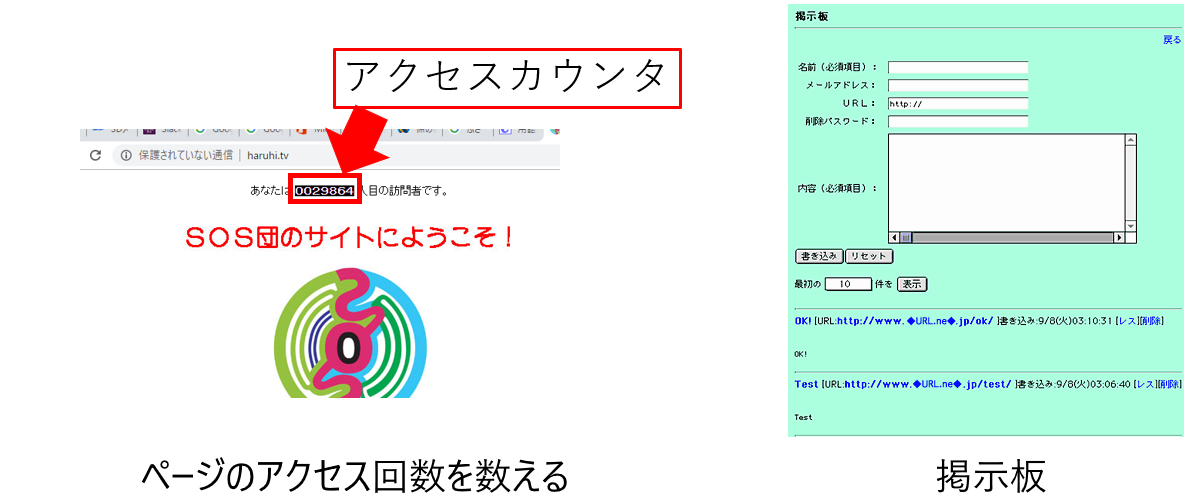
\includegraphics[width=\textwidth]{slide07-img008.png}}
        \end{minipage}
\end{frame}

\begin{frame}[fragile]
	\frametitle{CGIをりかいしよう:テキスト P.\pageref{1:P:CGI}-~~~\raisebox{-3mm}{
\includegraphics[width=0.1\textwidth]{raspberry}}}
        \begin{itemize}
            \item 第1回でつくった自己紹介ページのような、HTMLのみのWebページは毎回同じものが帰ってきます。
            \item HTML+CGIの場合、クライアントからの要求のたびにCGIプログラムがHTMLを作成するため、毎回違うWebページが返ってきます。
        \end{itemize}
        \begin{minipage}{\textwidth}
            {\upshape
              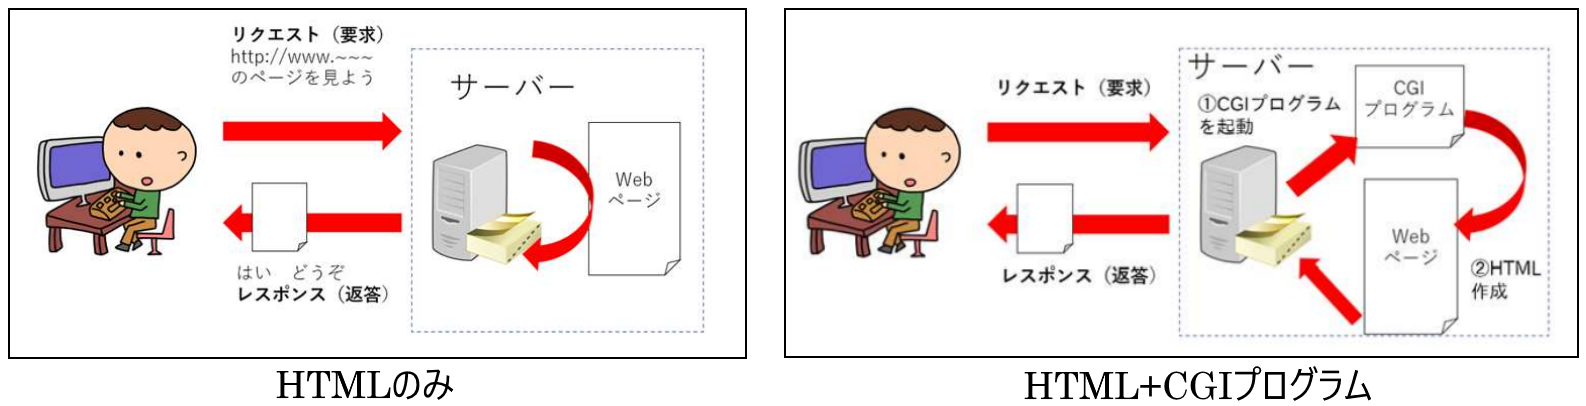
\includegraphics[width=\textwidth]{slide07-img010.png}}
        \end{minipage}
\end{frame}

\begin{frame}[fragile]
	\frametitle{CGIをつかってみよう:テキスト P.\pageref{1:P:CGI}-~~~\raisebox{-3mm}{
\includegraphics[width=0.1\textwidth]{raspberry}}}
      \large\textbf{教科書をよみながら、問題をやってみよう}
				\begin{itemize}
					\item \ref*{1:Q:dynamicPage}
					\item \ref*{1:E:CGI}
					\item \ref*{1:E:URL}
					\item \ref*{1:E:QS} 
				\end{itemize}
      \vfill
      \large\textbf{わからないことは、放っておかず、すぐに TA に聞きましょう}
\end{frame}

\end{document}
